\subsection{Vergleich von CAD-Viewer Programmen}
\label{subsec:comparison-cad-viewer}

Wir wollen die nachfolgend aufgelisteten, kostenlos verfügbaren, CAD-Viewer Programme testen.
Die Produkte sind durch eine Internetrecherche zum Thema CAD-Viewer aufgetaucht.

\begin{enumerate}
    \item Autodesk Viewer
    \item DWG TrueView
    \item eDrawings Viewer
    \item ABViewer
    \item DWG FastView
\end{enumerate}

Danach sollte eine Auflistung von Anforderungen möglich sein, die - neben den bereits gegebenen Anforderungen - für das neue Visualisierungswerkzeug für Gebäudepläne sinnvoll erscheinen.

\subsubsection{Autodesk Viewer}
\label{subsubsec:autodesk-viewer}

Das Programm \textit{Autodesk Viewer} vom ursprünglichen Entwickler des DXF-Formats Autodesk~\cite{DXFReference} ist eine web-basierte Lösung zur Ansicht von CAD-Dateien~\cite{AutodeskViewer}.
Zur Verwendung reicht ein Browser und ein Aufruf von https://viewer.autodesk.com sowie ein vorhandenes Benutzerkonto bei Autodesk.
Ein Screenshot davon ist in Abbildung~\ref{fig:autodesk-viewer} zu sehen.

Die Dateien zur Ansicht müssen dort hochgeladen werden.
Danach kann im Beispielgebäudeplan per Maus navigiert werden (Mausrad zum Anpassen des Maßstabs, Ziehen mit der Maus zum Verschieben).
Des Weiteren stehen Funktionen zum Messen zwischen verschiedenen Punkten und zum Markieren einer bestimmten Stelle oder eines Bereichs zur Verfügung.
Außerdem kann der Anwender den geöffneten Gebäudeplan im Rastergrafikformat PNG herunterladen.
In der resultierenden PNG-Dateien befinden sich auch alle vorgenommenen Markierungen und Messungen.

\begin{figure}
    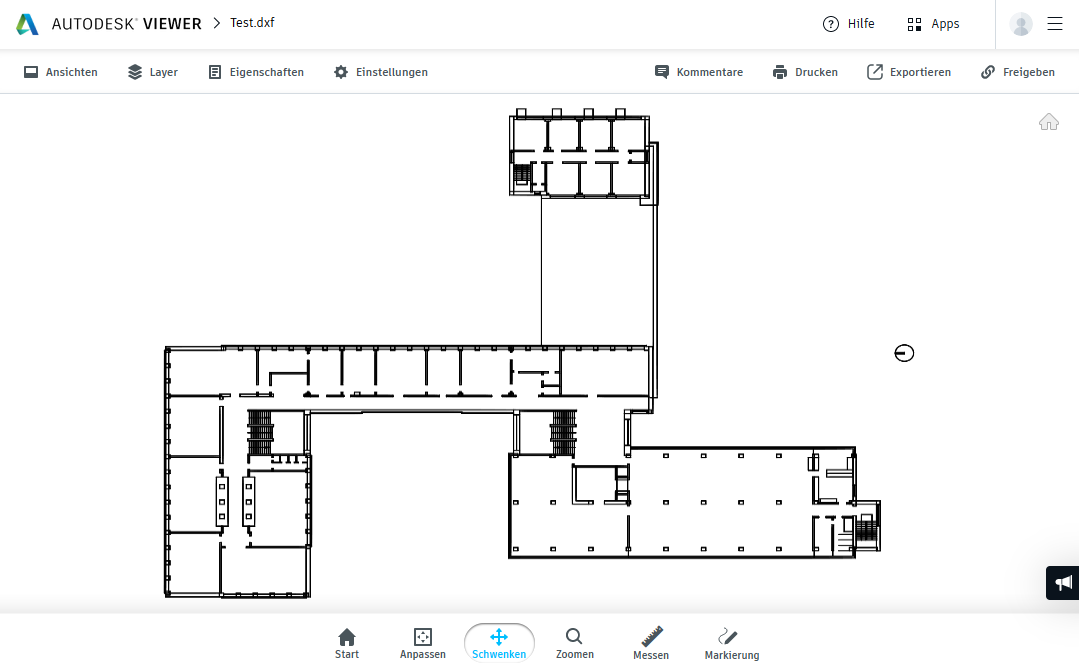
\includegraphics[width=0.5\textwidth]{res/autodesk-viewer.png}
    \caption{Screenshot des Programms \textit{Autodesk Viewer}.}
    \label{fig:autodesk-viewer}
\end{figure}
